\documentclass[8.01x]{subfiles}
\begin{document}

\chapter{Week 1}

\section{Lecture 1: Units, dimensions and scaling arguments}

The lecture begins with a quick intro to units, followed by a movie showing 40 orders of magnitude (from inside a proton, to a perspective 100 million lightyears from Earth).

After that, we begin talking about dimensional analysis and the metric system.
The three SI base units, and their respective dimensions, are introduced: the meter (m) for measuring length [L], the second (s) for measuring time [T] and the kilogram [kg] for measuring mass [M].\\
We use the square brackets to notate that we are not talking about a \emph{unit}, but a \emph{dimension} - such as the three shown above (length, time, mass), or speed, acceleration, temperature, charge, etc.\\
One dimension can have many units (meters, yards, kilometers, miles and light-years all describe length), but one unit always describes exactly one dimension. (If it were not so, we could perhaps measure temperature in meters, or length in amperes!)

As an important side note, keep in mind that capitalization is extremely important in physics: 1 mm is 1/1000 of a meter, a very short distance, while 1 Mm is a million meters, or 1000 kilometers - a distance larger than many countries. The same goes for units: k means kilo (the prefix for 1000), while K means Kelvin, a unit of absolute temperature. Capital $G$ is the symbol for the gravitational constant (about $6.67 \cdot 10^{-11} \text{ N(m/kg)}^2$), while a lowercase $g$ is the symbol for the gravitational acceleration near Earth, about $9.8 \text{ m/s}^2$. The two are related, but still completely different, so they must not be confused for one another.

Many other units can be described as combinations of the three base units shown above, for example:

\begin{equation}
 \text{[speed]} = \frac{\text{[L]}}{\text{[T]}}
\end{equation}

All units of speed are in length per time - meters per second, kilometers per hour, inches per year, etc. Therefore, we say that the \emph{dimension} of speed is the dimension of length per time, as shown above in a more mathematical notation.

Other examples are:

\begin{equation}
 \text{[volume]} =\text{[L]}^3
\end{equation}
\begin{equation}
 \text{[density]} = \frac{\text{[M]}}{\text{[L]}^3}
\end{equation}
\begin{equation}
 \text{[acceleration]} = \frac{\text{[L]}}{\text{[T]}^2}
\end{equation}

The last one may seem strange if you have not studied physics before - an example of a unit of acceleration is meters per second squared, or meters per second per second ($m/s^2$ or $(m/s)/s$). It's quite simple though, once you get past the wording of it.\\
When measuring a change in something, we always add another "per second" (or another unit of time), so when the unit we are measuring the change in is already meters per second, we get meters per second per second.\\
For example, a car might start out at 0 m/s (standing still), and be moving at 5 m/s one second later. In that case, the car's average acceleration is 5 meters per second per second.

\subsection{Uncertainty, and an experiment}
Prof. Lewin stresses very strongly: ``Any measurement you make without knowledge of its uncertainty is \emph{meaningless}''. He repeats this a few times throughout the lecture.

Using two rulers accurate to about $\pm$ 1 mm, he measures a student first standing up, and then lying down -- after measuring an aluminum bar, to show that the two rulers agree. They do, within 1 mm - the uncertainty.
The results of the experiment are a bit surprising: the student was about 2.5 cm $\pm$ 0.2 cm taller lying down! The reason being that gravity compresses our bodies slightly when standing up, while that effect would be gone lying down (since gravity then acts perpendicular to our length).

Because of the small uncertainty, compared to the relatively large height difference, we can be sure that the student indeed was taller lying down. Had the uncertainty of the measurement instead been $\pm 3$ cm, how could we know? The two values $185.7$ cm and $183.2$ cm are indistinguishable from each other if measured with a meter stick where the uncertainty is $\pm 3$ cm! The first could be anything between 182.7-188.7 cm, while the second could be anything from 180.2-186.2 cm. There is considerable overlap, which means the two could indeed be equal -- we could only know by making a more accurate measurement.

Calculating uncertainty properly can be quite complex, and the correct methods will not be taught or used in this class, as it is simply out of the scope. Instead, we use simplified methods, ``poor man's'' as the professor called them.

\subsubsection{Uncertainty in addition and subtraction}

For addition and subtractions, it couldn't be much easier: the uncertainty of the sum or difference is simply the sum of the two uncertainties:

\begin{equation}
 (A \pm a) + (B \pm b) = (A + B) \pm (a +b)
\end{equation}
\begin{equation}
 (A \pm a) - (B \pm b) = (A - B) \pm (a +b)
\end{equation}

You can find this result by calculating with the extremes. For example, for adding $1.5 \pm 0.003 \text{ m} + 3 \pm 0.005 \text{ m}$:

\begin{equation}
\text{min} = 1.497 \text{ m} + 2.995 \text{ m} = 4.492 \text{ m}
\end{equation}
\begin{equation}
\text{max} = 1.503 \text{ m} + 3.005 \text{ m} = 4.508 \text{ m}
\end{equation}

Both results are $0.008$ m away from $3 + 1.5 = 4.5$, and so the uncertainty is $\pm 0.008$ m, the sum of the two uncertainties.  
If we use the same method where we subtract, we will find the same result: the uncertainties \emph{add}, and the results will differ from the simple difference by $+0.008$ and $-0.008$, respectively.

\subsubsection{Uncertainty in multiplication and division}

First, keep in mind that some numbers are exact. If we multiply a length by 2 -- a constant, not a measurement -- then the length and the uncertainty are both multiplied by 2 exactly. No further work is necessary.\\
If the two are measurements, however, care needs to be taken.

One way to get a \emph{rough} uncertainty value when dividing is to choose the largest and smallest values, respectively, for the numerator and denominator, and then subtract the nominal value from that.\\
As an example, let's say we want to calculate the approximate gravitational acceleration of the Earth based on measurements of the time for an object to fall from a certain height. The equation used is

\begin{equation}
 g = \frac{2 h}{t^2}
\end{equation}

The 2 here is an exact value, so we don't need to worry about it.\\
If the height is $\SI{3.000(3)}{m}$ and the time taken is $\SI{0.781(2)}{s}$, we then find:

\begin{equation}
g = \frac{2\cdot\SI{3.000}{m}}{(\SI{0.781}{s})^2} \approx \SI{9.8367}{m/s^2} \approx \SI{9.84}{m/s^2}
\end{equation}

We can then calculate the uncertainty as mentioned above. For the numerator, we add the $+ 0.003$ m, and in the denominator, we subtract the $- 0.002$ s. Finally, we subtract the nominal value that we found above.

\begin{equation}
\text{error} = \frac{2 \cdot \SI{3.003}{m}}{(\SI{0.779}{s})^2} - g = \SI{9.8971}{m/s^2} - \SI{9.8367}{m/s^2} = 0.0604 \approx \SI{0.06}{m/s^2}
\end{equation}

There has not yet been an example with multiplication used in the course, but I would assume that you still try to find the maximum possible value (by choosing the maximum for both terms) and then subtract the nominal value, just as above.

\subsection{Scaling arguments and Galileo Galilei}

Long ago, Galileo Galilei asked himself: why are the mammals the sizes they are, and not much bigger? The short version of a possible answer he came up with is that if they were more massive, their bones would break. Below is a more detailed analysis of what he might have thought about.

Say we have a mammal. It has a size $S$ - very roughly defined, of course: there is no single length that defines the actual size of an animal properly. Let's just say that a mouse is perhaps 10 cm (plus the tail), and a horse is couple of meters -- and let's not worry about the details.

The animal has a thigh bone, or \emph{femur}, of length $\ell$, and a thickness $d$ (at the thinnest point). The cross-sectional area at that point is $A$. We can safely say that $A \propto d^2$ (A is proportional to d squared): doubling $d$ will multiply the cross-sectional area by 4.
We call the mass of the animal $m$.

\begin{center}
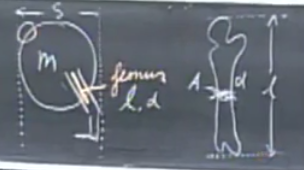
\includegraphics[scale=1.0]{Graphics/femur}
\end{center}

Let's now have a look at a scaling argument.\\
We assume that the length of the femur scales linearly with the size of the animal. That is, if the animal is twice as large as another, its femur will be twice as long as the other animal's femur. A reasonable assumption, one would think.

We then assume that the animal's mass is proportional to the cube of the size -- also very reasonable, as the size to the third is related to the animal's volume. Twice the volume, twice the mass, assuming the density is similar, of course.\\
Because of the previous relationship ($\ell \propto S$), this also implies that the mass is proportional to the length of the femur cubed. In mathematical notation, so far we have:

\begin{align}
 \ell &\propto S \label{eq:lproptoS}\\
 m &\propto S^3 \propto \ell^3 \label{eq:mproptoS3}
\end{align}

The \emph{pressure} on the femur is proportional to the weight of the animal, divided by the femur's cross sectional area. The weight (which the course will talk about later) is proportional to the mass, and as stated earlier, A is proportional to $d^2$, so we have

\begin{equation}
 \text{pressure} \propto \frac{m}{A} \propto \frac{m}{d^2}
\end{equation}

Because the bones will break if the pressure on them is too great, $m$ cannot increase without $d^2$ increasing by the same factor, if the animal is fairly close to the breaking limit already. This is key in this argument.

Because of this, we find
\begin{equation}
m \propto d^2 \label{eq:mproptod2}
\end{equation}

... or the above cannot be true.
Combining equation \eqref{eq:mproptoS3} with equation \eqref{eq:mproptod2} just above, we find

\begin{equation}
 d^2 \propto \ell^3
\end{equation}
or, taking the square root of both sides,
\begin{equation}
 d \propto \ell^{3/2} \label{eq:dproptoell32}
\end{equation}

The above is the result we have been looking for. What this means is that if we have two animals, one being 10 times larger than the other ($S$ being 10 times larger, which implies $\ell$ being 10 times larger via \eqref{eq:lproptoS}, via the above relation, the diameter of the femur $d$ must be $10^{3/2} \approx 32$ times greater!\\
If we compare e.g. a mouse and an elephant, the difference in size being perhaps 100 times, via the same relationships, $d$ must be $100^{3/2} = 1000$ times greater for the elephant!

Galileo Galilei may have thought this to be a good explanation as to why mammals are the size they are, and not much bigger: much larger animals would have bones so large, that they barely consist of anything else than bones to hold their weight up. Let's see if this appears to be correct by making some calculations on actual measurements of animal femurs.

If we take equation \eqref{eq:dproptoell32} and divide both sides by $\ell$, we find

\begin{equation}
\frac{d}{\ell} \propto \sqrt{\ell}
\end{equation}

This is then plotted from the professor's measurements of the bones. If the above is correct, we would expect that if $\ell$ is 4 times greater (such as a horse vs a raccoon), $d/\ell$ should be $\sqrt{4} = 2$ times greater.

The professor then showed the result of the experiment, by measuring these values ($d$ and $\ell$) for bones from various animals: a mouse, an opossum, a raccoon, an antelope, a horse, and an elephant. There was no evidence that the ratio of $d/\ell$ was different as we would have been expected. Even for the case of a mouse vs an elephant, where the difference in size (and thus $\ell$) would be about a factor of 100, so that we expect $d/\ell$ for the elephant to be about 10 times greater than for the mouse, we find less than a factor of two!\\
Similar relationships were shown between all animal sizes: in no case was $d/\ell$ significantly different, as the hypothesis predicted. It looks like we, and Galilei, must admit defeat. The hypothesis simply doesn't hold up to experiment!

\subsection{Dimensional analysis}

Let's now look at some basic kinematics (the physics of motion) and dimensional analysis in closer detail.\\
We drop an object, such as an apple, from a height $h$, and use a stopwatch to measure the time $t$ before it hits the ground. How does the time $t$ relate to the height $h$?

We can assume that the time is proportional to the height, to some unknown power, which we will call $\alpha$:

\begin{equation*}
 t \propto h^\alpha
\end{equation*}

The mass of the apple might matter, so we might expect to find it to be proportional to the mass to some unknown power $\beta$:

\begin{equation*}
 t \propto h^\alpha m^\beta
\end{equation*}

Finally, it might be related to the Earth's gravitational acceleration $g$ (not to be confused with the gravitational constant $G$; both of these will be introduced properly later in the course):

\begin{equation}
t \propto h^\alpha m^\beta g^\gamma
\end{equation}

We can now start trying to figure this out. We know that the left-hand side has the dimension of time, [T]. This means that the product on the right-hand side must also have the dimension of time. Using the dimensional analysis notation, we must have

\begin{equation}
 \text{[T]}^1 = \text{[L]}^\alpha \text{[M]}^\beta \left( \frac{\text{[L]}}{\text{[T]}^2} \right)^\gamma 
 \end{equation}
 ... where we have simply replaced the variable names with their respective dimensions, the dimension of $h$ being length, $m$ being mass, and $g$ being acceleration (length per time${}^2$).
 
 We can now start working. There is only one [M] in this equation, and it's on the right-hand side. There is no possible way to get it to cancel out with anything else, so $\beta$ must be 0 so that it disappears ``by itself'', so to speak.
 
 We have two [L] on the right hand side, but there is no [L] on the left-hand side. That means that the two must cancel each other out, in one way another. That is,
 
\begin{equation*}
 \alpha + \gamma = 0
\end{equation*}

must be true.

Finally, we have [T] to the power one on the left-hand side, and to the power $-2\gamma$ (since it is in the denominator, it is negative) on the right-hand side, and the two must be equal. All in all, we find

\begin{align*}
\beta &= 0\\
\alpha + \gamma &= 0\\
-2\gamma &= 1
\end{align*}

We can solve the last equation for $\gamma$, and stick that value into the second equation, to find the final answers:

\begin{align*}
-2\gamma &= 1\\
\gamma &= -\frac{1}{2}
\end{align*}

\begin{align*}
\alpha - 1/2 &= 0\\
\alpha = \frac{1}{2}
\end{align*}

And, so, we find these values, and these relationships with the variable names we had chosen earlier:

\begin{align}
t &\propto h^{1/2} g^{-1/2} \\
t &\propto \sqrt{\frac{h}{g}}
\end{align}

Since the meaning of a proportionality is that some (still unknown) constant multiplies the value, we can write this as an equality with an unknown constant $C$:

\begin{equation}
 t = C \sqrt{\frac{h}{g}}
\end{equation}

So, since the time is proportional to the square root of the height, we can tell than if we drop an object first from 2 meters, and then from 8 meters, it will take twice as long to fall the second time, despite the distance being 4 times as long (because $\sqrt{4} = 2$).

\subsection{An experiment}

This is then put to the test in the lecture, by dropping apples, and timing their fall. One drop was from 3 meters, $\pm 0.003$ meters, while the second was from 1.5 meters, also with $\pm 0.003$ meters as the uncertainty.

The ratio between the two is easily calculated as 2, but what about the uncertainty? If the numerator were $3.003$ m and the denominator $1.497$ m, those would give the largest ratio possible with the uncertainty of $\pm 0.003$. The result of that division is $2.006$, so we consider the uncertainty to be $0.006$:

\begin{equation}
 \frac{h_1}{h_2} = \frac{3.000 \pm 0.003 \text {m}}{1.500 \pm 0.003 \text{ m}} = 2.000 \pm 0.006
\end{equation}

Note that because this is a ratio between two lengths, the end result has no dimension and thus no unit.

Knowing this ratio, we can now predict the ratio between the fall times. Since the ratio between the heights is 2, and the time is proportional to the square root of the height, the ratio between the fall times should be about $\sqrt{2}$. Then there's that uncertainty again. We can use the same method to find the smallest possible and the largest possible result by calculating $\sqrt{2+0.006}$ and $\sqrt{2-0.006}$ and will find an uncertainty of about $\pm 0.002$. That gives us

\begin{equation}
 \frac{t_1}{t_2} = \sqrt{\frac{h_1}{h_2}} = 1.414 \pm 0.002 \label{eq:applepred}
\end{equation}

So, the above is our \emph{prediction}, and we have a set-up with the apple fall times being measured automatically. Let's see the results!

The apple falling from 3 meters $\pm 3$ mm took $0.781 \pm 0.002$ seconds to fall. The apple falling from 1.5 meters $\pm 3$ mm took $0.551 \pm 0.002$ seconds to fall.

If we then calculate the ratio between the two times, we find

\begin{equation}
\frac{0.781 \pm 0.002}{0.551 \pm 0.002} = 1.417 \pm 0.008
\end{equation}

... which is in agreement with the prediction in \eqref{eq:applepred} when we consider the uncertainties in our measurements. \emph{Physics works}, as Prof. Lewin would say.\\
As far the uncertainty of the above result goes, I get $\pm 0.009$ when calculating the same way as before. However, as mentioned before, this method is not truly correct, and the truly correct way is out of the scope of this course, so such a small difference does not matter.\\
As long as the uncertainty is 0.001 or more, the results can agree with each other.

\section{Lecture 2: Introduction to Kinematics}

\subsection{Distance vs displacement and velocity vs speed}

In everyday English, speed and velocity are usually used as synonyms. In physics, however, the two are very different, and it's important to understand the difference.\\
We can define the two as

\begin{align}
 \text{speed} &= \frac{\text{distance traveled}}{\text{time taken}}\\
 \text{velocity} &= \frac{\text{displacement}}{\text{time taken}}
\end{align}

On first glance, the two may appear to say the same thing, but they don't.\\
There is an important difference between the terms \emph{distance traveled} and \emph{displacement}. The first is a scalar, and is always positive (if not zero, if you have been standing still the entire time) and is equal to what a car's odometer would display.\\
Displacement, however, is a \emph{vector} (see Part I on vector mathematics, or lecture 3). It is the distance between the starting point and the ending point - which may be zero, if you've traveled back to the start.\\
The displacement vector, like all vectors, also has a direction, which is defined as pointing from the starting point to the ending point.\\
With this in mind, it should be clear that the distance traveled must \emph{always} be greater than or equal to the displacement. Anything else would require teleportation!

Now, consider the case where we travel 1 km due north, turn around, and travel 1 km due south. We have traveled 2 km, but we are still standing exactly where we started! In other words, the displacement is zero. Using the above definitions, our average \emph{velocity} for the entire journey was \emph{zero} -- zero displacement divided by any measured time is zero.\\
The average \emph{speed}, on the other hand, is guaranteed to be positive, and can be found by dividing the 2 kilometers traveled by the time the journey took.

There is another difference between the two: speed is a scalar, that is, a regular number like any other. Velocity, on the other hand, like displacement, is a vector.\\
The average speed for the first half of the journey (right where we turned around) might have been 10 m/s, while the average velocity at that point might have been 10 m/s to the north.

Vectors are introduced properly in the first part of these notes, and in the next lecture of the course as well.

\subsection{Kinematics}

\begin{center}
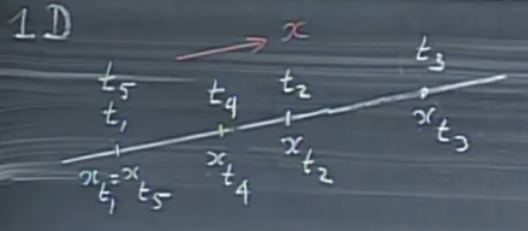
\includegraphics[scale=0.75]{Graphics/1d-motion}
\end{center}

The increasing direction of $x$ is as shown. An object moves along this line, first towards the right, then shortly after reaching the point $x_{t3}$ at  $t = t_3$, it reverses and moves back, until it is at $x_{t1} = x_{t5}$, where it started.

We can now introduce a definition for the \emph{average velocity} of this object between two times $t_1$ and $t_2$ as the following:

\begingroup
\large
\begin{equation}
 \overbar{v}_{t_1 t_2} = \frac{x_{t2} - x_{t1}}{t_2 - t_1}
\end{equation}
\endgroup

This should make some intuitive sense -- the numerator is just the distance between the two points (the \emph{displacement}), while the denominator is the time that has passed. Displacement over time gives us the \emph{average velocity}.

If we consider the average velocity between times $t_1$ and $t_5$, the answer is zero, because the position is the same for the two times, and so we have zero divided by the time taken, which is of course simply zero.\\
Between e.g. times $t_2$ and $t_4$, the velocity is \emph{negative}, which indicates we have moved in the \emph{opposite direction} of the positive $x$ axis.\\
The average velocity can be positive, zero or negative, depending on the positions involved.\\
The average \emph{speed}, however, is \emph{always} positive or zero. The average \emph{velocity} is still zero, because the distance between the starting point and the ending point is zero.

\begin{center}
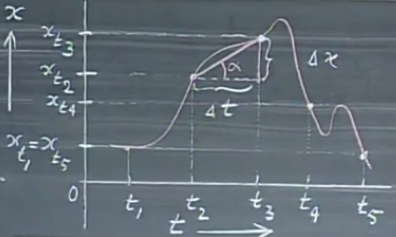
\includegraphics[scale=0.75]{Graphics/1d-motion-graph}
\end{center}

Here, we see a different way of notating what is really the same thing as we have above. If we call a difference in time $\Delta t$, and a difference in $x$ position $\Delta x$, we can find the average velocity as

\begin{equation}
 \overbar{v} = \frac{\Delta x}{\Delta t}
\end{equation} 

This is simply a different way of notating what we already had. Be careful with signs, though - if you take the first $x$ value in the middle, and the second from the right, be sure to take the $t$ values in the same order, or you will get the negative of the correct answer. In other words, your average velocity will be in the opposite direction of the actual movement.

Also shown above is the angle $\alpha$, that we can find between two arbitrary points. When $\alpha > 0$, as above (it's pointing upwards), the average velocity is positive. If it is instead negative, as it would be between $t_4$ and $t_5$, the average velocity is negative.

\subsubsection{Instantaneous velocity}

Since the definition of velocity we've seen thus far is only an average between two points in time, what is the meaning of instantaneous velocity (which is usually what we mean by ``velocity'' unless otherwise specified)?\\
Conceptually, the answer is that it is still an average, only that we move the two position measurements closer and closer together in time, until the time between them is zero.

Mathematically, velocity is the first \emph{derivative} of position.
We could write it as

\begingroup
\large
\begin{equation}
 v_t = \lim_{\Delta t \to 0} \frac{x_{t + \Delta t} - x_t}{\Delta t} = \frac{dx}{dt} = x'(t) = \dot{x}
\end{equation}
\endgroup

The last three are just three different ways of writing the same thing: the first derivative of $x$ with respect to $t$. Leibniz' notation looks like a fraction; Lagrange's notation uses the prime symbol (apostrophe) to indicate a derivative, and finally Newton's notation uses a dot above to signify the first time derivative. (In other words, the dot notation is used almost exclusively when the function is differentiated with respect to time, so the $t$ is implicit.)

As for speed, we can simply define instantaneous speed as the absolute value of the instantaneous velocity. In other words, if the velocity has a minus sign, remove it. If not, the two are equal.

\subsection{Calculating the average speed of a bullet}

Using an electronic, an experiment was set up to measure the speed of a bullet. The bullet is fired from a rifle, and breaks a wire, at which point the timing starts. Soon thereafter, the same bullet breaks another wire, at which point the timing stops.

Using a measurement of the distance, and a measurement of the time taken, we can calculate the average speed.

The distance was measured to be $148.5 \pm 0.5$ cm, that is, $1.485 \pm 0.005$ m.\\
The time taken was measured as $5.8 \pm 0.1$ ms, which equals, $0.0058 \pm 0.0001$ s.

The average speed is then

\begin{equation}
v_{avg} = \frac{\SI{1.485}{m}}{\SI{0.0058}{s}} = \SI{256}{m/s}
\end{equation}

The relative error in the timing can be calculated as 

\begin{equation}
\text{relative error} = \frac{\SI{0.1}{ms}}{\SI{5.8}{ms}} \cdot 100\% = 1.7\% 
\end{equation}

The uncertainty in the average speed can then be estimated. As the lecture question hints, we will ignore the uncertainty due to error in the distance measurement, because the timing error is much greater.

We can use the simple way introduced previously to find an approximate uncertainty:

\begin{equation}
\text{error} = \frac{1.485 \text{ m}}{0.0058 - 0.0001 \text{ s}} - \SI{256}{m/s} = \SI{4.5}{m/s}
\end{equation}

(We would add $+0.005$ m at the top, if we didn't choose to ignore the uncertainty it that measurement.)\\
Alternatively, we could have simply used the 1.7\% relative error we found above.\\
So in short, we can specify the average speed of the bullet as

\begin{equation}
v_{avg} = 256 \pm 4.5 \text{ m/s}
\end{equation}

\subsection{Acceleration}

Just as velocity is the change in position, acceleration is the change in \emph{velocity}. We can use an equation that looks extremely similar to find the \emph{average} acceleration $a$:

\begingroup
\large
\begin{equation}
 \overbar{a}_{t_1 t_2} = \frac{v_{t2} - v_{t1}}{t_2 - t_1}
\end{equation}
\endgroup

The dimension of acceleration, as mentioned previously, is length per time${}^2$, or [L] [T]${}^{-2}$, with $\text{m/s}^2$ being the most common unit, at least in this course.

Just as before, we can simplify this by using delta notation, with the same caveat: make sure to use the correct signs, or the result may end up incorrect.

\begin{equation}
\overbar{a} = \frac{\Delta v}{\Delta t}
\end{equation}

As an example, let's use the following lecture question. We define the direction of increasing $x$ as upwards (towards the sky). A tennis ball is thrown towards the ground at a velocity of about $\SI{-5}{m/s}$ - i.e. the speed is 5 m/s, downwards. It is in contact with the ground for about 1/100 second, after which it is moving at $\SI{+5}{m/s}$, i.e. upwards.\\
What is the average acceleration of the tennis ball?

Well, we have the formula above, so this should be fairly easy!

\begin{equation}
 \overbar{a_{ball}} = \frac{\SI{5}{m/s} - (\SI{-5}{m/s})}{\SI{0.01}{s}} = \frac{\SI{10}{m/s}}{\SI{0.01}{s}} = \SI{1000}{m/s^2}
\end{equation}

Keeping the signs in mind, we end up with a positive value for the acceleration, which has a ridiculous magnitude - over 100 times the Earth's gravitational acceleration.

The professor adds another example of acceleration. There is a limit to the amount of acceleration things can tolerate before they break. He used examples of tomatoes and eggs, also thrown to the ground at 5 meters per second.\\
The impact time will probably be much greater (perhaps 1/4 second), and the change in velocity will be only 5 m/s rather than 10, as neither the egg nor the tomato would bounce back up.\\
Despite that, clearly, both would break, even though the acceleration is a more modest $20 \text{ m/s}^2$ or so.

The next example was that of a human skull on a marble floor, from a Sherlock Holmes movie. Even at a relatively small velocity, a skull hitting such a hard floor, with no ``give'', the impact time would be extremely short. Since the impact time is in the denominator, a shorter time will result in a higher acceleration, and a skull can break despite the low speeds involved. 

\subsubsection{Instantaneous acceleration}

Just as we did with velocity, we now want a way to calculate the acceleration at a given instant, rather than the average between two measurements. We do this in exactly the same way: we find the first time derivative of the velocity.

\begingroup
\large
\begin{equation}
 a_t = \lim_{\Delta t \to 0} \frac{v_{t + \Delta t} - v_t}{\Delta t} = \frac{dv}{dt} = \frac{d^2x}{dt^2} = \ddot{x}
\end{equation}
\endgroup

We could also write this as $x''(t)$ or $v'(t)$, but I wanted to reduce the amount of clutter above somewhat.\\
Since acceleration is the time derivative of velocity, and velocity itself is the time derivative of position, acceleration is the \emph{second} time derivative of position, as shown above.

\subsection{General forms for one-dimensional motion}

We can write equations for the position and velocity in one-dimensional motion in such a way that they can be used for \emph{any} one-dimensional motion with a constant acceleration:

\begin{align}
x(t) &= x_0 + v_0 t + \frac{1}{2} a_x t^2\\
v(t) &= v_0 + a_x t
\end{align}

... where $x_0$ is the initial $x$ position, $v_0$ is the initial velocity, and $a_x$ is the acceleration in the positive $x$ direction.\\
Each of these three numbers can independently be negative, zero, or positive, and produce valid physical situations.\\
The same formula can be used in a situation with a constant velocity: simply set $a_x = 0$, and the equations are valid. (The second equation becomes trivial, of course, so only the equation for $x(t)$ will be useful.)

\section{Lecture 3: Vectors}

Because I had already written the part on vector mathematics in these notes long before this course started (I did it about a year ago, when I considered taking 8.01 via MIT OCW), most notes from this lecture are in that part instead.

However, I do find it useful to talk about one thing that is more specific to physics than the vector mathematics part, and that is vector decomposition. Perhaps not decomposition in itself, but the consequences of it for simplifying 2- or 3-dimensional kinematics.

If we have a position vector $\vec{r_t}$, which changes with time:

\begin{align}
 \vec{r_t} &= x_t \hat{x} + y_t \hat{y} + z_t \hat{z} \\
 \vec{v_t} = \frac{d\vec{r_t}}{dt} &= \dot{x} \hat{x} + \dot{y} \hat{y} + \dot{z} \hat{z}\\
 \vec{a_t} = \frac{d\vec{v_t}}{dt} &= \ddot{x} \hat{x} + \ddot{y} \hat{y} + \ddot{z} \hat{z}
\end{align}
... using Newton's notation, with a dot representing the first time derivative, and two dots representing the second time derivative.

We could use these three equations as they stand, to calculate the position, velocity and acceleration of a particle in three dimensions. However, that would likely get complex very quickly.

What we can instead do is break the three-dimensional motion into multiple one-dimensional motions.\\
Imagine we throw a ball, sideways. Its motion will be constrained to two dimensions, if we neglect wind and air drag: it will start accelerating downwards due to gravity, and it will move horizontally in the direction we threw it at constant velocity. The latter is important: gravity only accelerates the ball downwards. If we neglect wind and air drag, as mentioned, there is no force acting on the ball parallel to the ground. Because of Newton's first law (which we have not yet introduced, but will next week), that means the velocity must be constant in that direction.

Thus, we have reduced a fairly complex problem of three-dimensional motion into \emph{two} problems of one-dimensional motion. One horizontally, where the velocity is constant, and one vertically, where gravity acts as a constant acceleration downwards.

\newpage

\subsection{3-dimensional motion to two independent 1-dimensional motions}

Let's examine the problem of a ball (or a similar object) being thrown diagonally upwards. If there is no air, and thus no wind that could cause the ball to curve, the motion will be constrained to two dimensions, despite moving in three-dimensional space.\\
We can therefore think of this as a 2D problem, where the ball moves along this trajectory:

\begin{center}
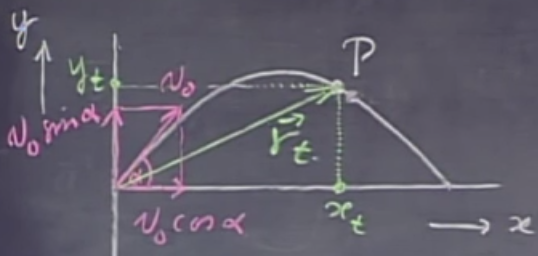
\includegraphics[scale=0.65]{Graphics/2d-motion-decomposed}
\end{center}

The ball moves along the trajectory shown in white. It is launched (thrown) at an initial velocity $v_0$ (in magenta), which is a vector pointing at an angle $\alpha$ from the ground. Also in magenta, we have the initial velocities for the $x$ and $y$ directions, found via vector decomposition:

\begin{align}
v_{0x} &= v_0 \cos \alpha\\
v_{0y} &= v_0 \sin \alpha
\end{align}

Because there is no force acting on the ball in the $x$ direction, this is the velocity it will have in the $x$ direction until it hits the ground.\\
In green, the ball's position vector at a later point is shown, together with its $x$ and $y$ components, all three dependent on time $t$.

We can now apply the equations we found earlier, for one-dimensional motion under either constant acceleration or constant velocity. That is, these:

\begin{align}
x(t) &= x_0 + v_{0x} t + \frac{1}{2} a_x t^2\\
v_x(t) &= v_{0x} + a_x t
\end{align}

The same equations can of course be used for $y$ (and $z$) by simply replacing all $x$ terms with $y$ (or $z$).

With these equations in mind, we can now calculate the object's $x$ position at any moment in time as

\begin{equation}
x(t) = (v_0 \cos \alpha) t
\end{equation}

... since we are free to choose $x_0 = 0$, and there is no acceleration in the $x$ direction ($a_x = 0$).

This simple equation describes the $x$ position completely, from $t=0$ when it is launched, to whenever it hits the ground. To find out when that is, we need to calculate the $y$ position over time.

We use the same equations, with $y_0 = 0$	 (again, we are free to choose where we place our zero coordinate), and $a_y = -g$, that is, the gravitational acceleration of the Earth. $g$ is always positive, however, and in the diagram, we have chosen increasing $y$ to be upwards. Therefore we need to be careful and write $-g$ in this case, or we would be saying that gravity would accelerate the ball towards the sky!

We make the substitutions for the values ($y_0$ and $a_y$ as mentioned above, and the initial velocity in the $y$ direction is $v_0 \sin \alpha$ as we saw before)

\begin{align}
y(t) &= (v_0 \sin \alpha) t - \frac{1}{2} g t^2\\
v_y(t) &= v_0 \sin \alpha - g t
\end{align}

Note the minus sign for the acceleration.\\
The last three equations completely describe the ball's $x$ position, $y$ position, and $y$ velocity. The $x$ velocity is known to be constant.

Together, we can use the $x(t)$ and $y(t)$ equations to describe the trajectory:

\begin{align*}
x(t) &= (v_0 \cos \alpha) t\\
y(t) &= (v_0 \sin \alpha) t - \frac{1}{2} g t^2
\end{align*}

This is then demonstrated in lecture, by firing a golf ball straight up (as seen by the launcher), from a cart moving on a rail.\\
For an outside observer, such as us, the ball moves in a parabolic trajectory, and returns to the launcher a few seconds later, as they moved together at the constant $x$ velocity.\\
The successful demonstration concludes this lecture.

\end{document}